\documentclass[accentcolor=tud9c,colorbacktitle,inverttitle,landscape,german,presentation,t]{tudbeamer}
\usepackage{ngerman}
\usepackage{subcaption}
\usepackage{graphicx}
\usepackage{pgfplots}
\usepackage{pgfplotstable}



\begin{document}

\title{\"Ubung 5}
\subtitle{Visual Computing - Bilder}

\author[Johannes Beck, Christian Eilers, Robin Menzenbach, Martin Steinborn]{Johannes Beck, Christian Eilers, Robin Menzenbach, Martin Steinborn}

%\institute[IFP TUD]{Institut f"ur Festk"orperphysik, TU Darmstadt}

%\logo{\includegraphics{TUDbeamer-logo}}
% \logo{\color{tudtextaccent}\large IFP}

\date{\today}

\begin{titleframe}
\end{titleframe}

\section{Aufgabe 1}
	\begin{frame}
		\frametitle{Aufgabe 1: Tiefpass vs. Hochpass \\ a)}
		Bei dem ersten angegebenen Amplitudenspektrum handelt es sich um eienn Tiefpass-Filter. Dies ist is leicht daran zu erkennen, dass niedrige Frequenzen ungehindert passieren k\"onnen, w\"ahrend hohe vollst\"andig geblockt werden.
		Das zweite Amplitudenspektrum kann einem Hochpassfilter zugeordnet werden, da hier hohe Frequenzen ungest\"ort passsieren, w\"ahrend niedrige geblockt werden.
	\end{frame}
	
	\begin{frame}
	\frametitle{Aufgabe 1: Tiefpass vs. Hochpass \\ b)} %TODO Anwendungsfälle
	Ein Tiefpassfilter zeichnet sich dadurch aus, dass er hohe Frequenzen blockt und niedrige passieren l\"asst. Als Schaltbedingung gilt hierbei
	\begin{align*}
	H(\omega) = \left\{\begin{array}{rl}0 & \textrm{f\"ur} \mid\omega\mid < \omega_1 \\ 1 & \textrm{f\"ur} \mid\omega\mid \geq \omega_1	\end{array}\right. .
\end{align*}
	Anwendung findet er besonders, da das Abschneiden der hohen Frequenzen  eine Unterdr\"uckung von Rauschen zufolge hat. Allerdings kommt es zu einer generellen Zunahme an Unsch\"arfe, sogenannt blur-Effekt.	\\	
	
	Der Hochpassfilter wirkt genau anders herum. Er schneidet tiefe Frequenzen ab und l\"asst hohe passieren. dies hat zur Folge, dass scharfe \"Uberg\"ange deutlicher hervortreten. Als Schaltbedingung gilt hier
	\begin{align*}
	H(\omega) = \left\{\begin{array}{rl}1 & \textrm{f\"ur} \mid\omega\mid < \omega_1 \\ 0 & \textrm{f\"ur} \mid\omega\mid \geq \omega_1	\end{array}\right. .
\end{align*}	
	\end{frame}

	\begin{frame}
	\frametitle{Aufgabe 1: Tiefpass vs. Hochpass \\ c)}
	Die dritte Filterart ist der sogenannte Bandpass-Filter. Er l\"asst alle Frequenzen $\omega$ innerhalb eines bestimmten Gebietes, Band genannt, passieren. Damit folgt f\"ur die Schaltfunktion
	
	\begin{align*}
	H(\omega) = \left\{\begin{array}{rl}1 & \textrm{f\"ur } \omega_1 < \omega < \omega_2 \\ 0 & \textrm{sonst} \end{array}\right. .	
\end{align*}	

Das beispielhafte Amplitudenspektrum eines Bandpasses, welches auf der n\"achsten Folie abgebildet ist, zeigt deutlich, wie nur eine bestimtme Bandbreite an Frequenzen passieren kann und alle gr\"o\ss eren und kleineren geblockt werden. Die Breite der passierenden Frequenzen ist dabei je nach Bandpass verschieden. 
\end{frame}

\begin{frame}
\frametitle{Aufgabe 1: Tiefpass vs. Hochpass \\ c)}

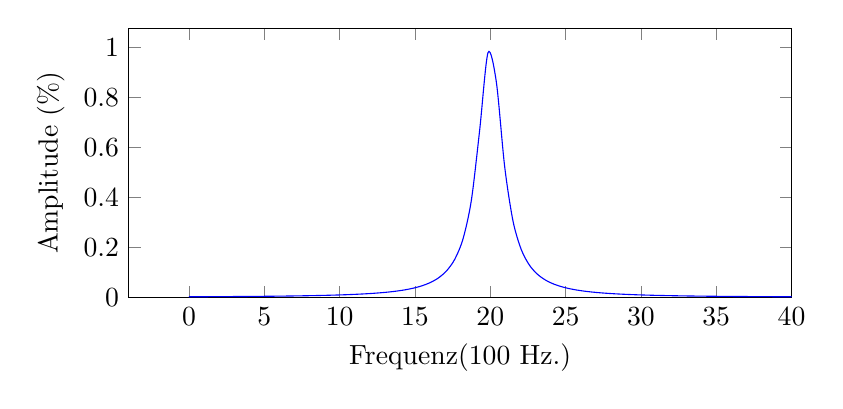
\begin{tikzpicture} 
\begin{axis}[domain=0:220,
			smooth,
			samples=400,
			height=5cm,
			width=10cm,
			ymin=0, 
			xmax=40,
			ytick={0,0.2,...,1},
			xlabel=Frequenz(100 Hz.), 
			ylabel=Amplitude (\%)] 
\addplot[color=blue,mark=]{1/((x-20)^2*1 +1)};

 \end{axis}

 \end{tikzpicture}
	\end{frame}
	
\section{Aufgabe 2}
	\begin{frame}
		\frametitle{Aufgabe 2: Pixeloperation und Filtermasken \\ a)}
			\label{2_a}
			Pixel-Operation und Filtermasken unterscheiden sich darin, dass bei Pixel-Operationen das zu bearbeitende Pixel ohne Einfluss der Pixel in seiner Umgebung bearbeitet wird. Seine Nachbarschaft spielt also keine Rolle. Bei Filtermasken ist dies exakt anders herum. hier werden Pixel in Abh\"angigket ihrer Nachbarschaft bearbeitet. Es spielt also nicht nur eine Rolle wie das entsprechende Pixel aussieht, sondern auch wie es um es herum aussieht.
	\end{frame}

	\begin{frame}
		\frametitle{Aufgabe 2: Pixeloperation und Filtermasken \\ b)}
		%TODO Hab ich gegoogelt, bin mir aber net sicher
		Das Problem von Filtermasken bei der Verwendung am Rande eines Bildes besteht darin, dass sie wie zuvor beschrieben nicht nur auf das zu bearbeitende Pixel zugreifen um es  zu ver\"andern, sondern auch um die Pixel in der direkten Nachbarschaft. Dies gechieht in alle Richtungen gleicherma\ss en und somit entsteht das Problem, dass am Rand eine Richtung keine benachbarten Pixel mehr hat und somit die Filttermaske auf nicht existierende Pixel zugreifen m\"usste. Zwei m\"ogliche L\"osungen dieses Problems sind zum Beispiel am Rand keine Filter anzuwenden. Dadurch g\"abe es keine Zugriffe au\ss erhalb der Daten und das Problem w\"are gel\"ost. Als zweite Option k\"onnte man den letzten verf\"ugbaren Wert benutzen der korrekt bearbeitet werden konnte, um unzul\"assige Zugriffe zu vermeiden. 
	\end{frame}
	
	\begin{frame}
		\frametitle{Aufgabe 2: Pixeloperation und Filtermasken \\ c)}
		%TODO soll man hier rand und filter getrennt angeben und passst das mit der randmethode?
	
		Die Anwendung eines 3x3 Mittelwert-Filters auf das gegebene Graustufenbild liefert
		\begin{align*}
		\begin{bmatrix}
		230 & 15 & 220 & 158 & 100 \\
		156 & 131 & 115 & 111.444 & 19\\
		7 & 111.444 & 115.333 & 98.333 & 103\\
		88 & 103.222 & 121.778 & 106.333 & 73\\
		142 &234 & 67 & 186 & 28
		\end{bmatrix}
		\end{align*}
		als Ergebnis. Zur Randbehandlung wude die Methode gew\"ahlt, am Rand keinen Flter anzuwenden. Die Ergebnisse der Randes sind somit dieselben wie vor der Anwendung des Filters, w\"ahrend alle restlichen Werte sich ver\"ndert haben, wie in dem neuen Graustufenbild zu sehen ist.
	\end{frame}

\section{Aufgabe 3}
	\begin{frame}
		\frametitle{Aufgabe 3: Digitale Kamera \\ a)}
		%TODO 3a)
	\end{frame}
	
	\begin{frame}
		\frametitle{Aufgabe 3: Digitale Kamera \\ b)}
		%TODO 3b)
	\end{frame}
	
	\begin{frame}
		\frametitle{Aufgabe 3: Digitale Kamera \\ c)}
		%TODO 3c)
	\end{frame}
\section{Aufgabe 4}
	\begin{frame}[t]
		\frametitle{Aufgabe 4: Histogrammausgleich}
		\begin{figure}
		\centering
		\begin{minipage}[c]{.2\textwidth}
			\centering
			$\begin{bmatrix}
			6& 48& 94& 33& 7\\
			12& 36& 26& 71& 91\\
			29& 17& 34& 45& 67\\
			34& 55& 74& 1& 41\\
			87& 14& 28& 61& 32
			\end{bmatrix}$
		\end{minipage}
		\qquad \qquad
		\begin{minipage}[c]{.2\textwidth}
			\centering
			$\huge\Rightarrow$
		\end{minipage}
		\begin{minipage}[c]{.3\textwidth}
			\centering
			$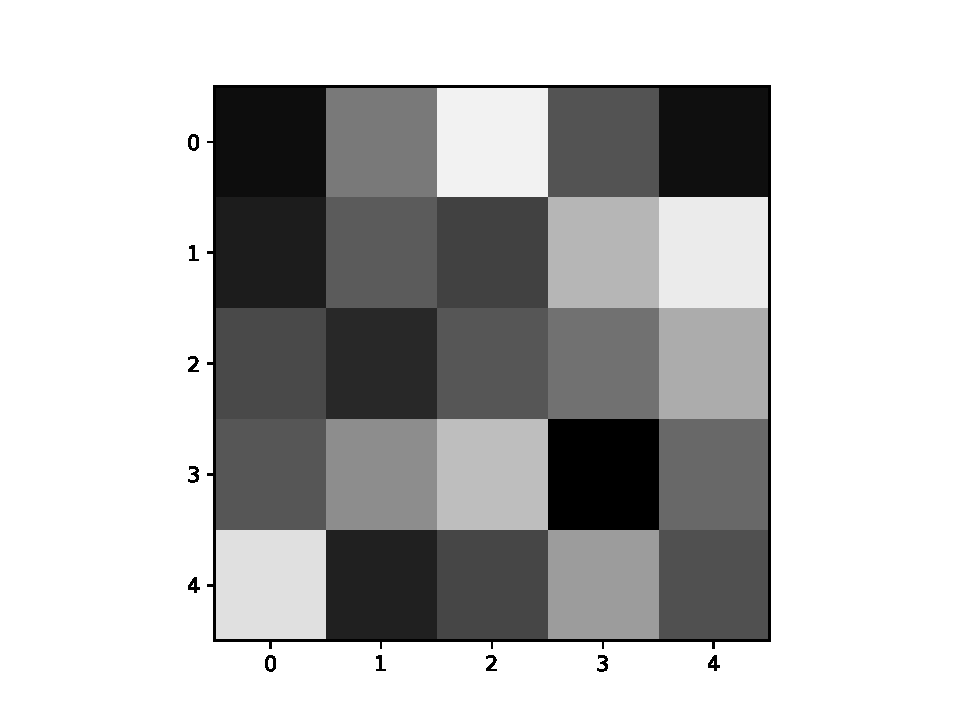
\includegraphics[width=\textwidth]{fig/image.pdf}$
		\end{minipage}
		\end{figure}

		
	\end{frame}
	\begin{frame}[t]
		\frametitle{Aufgabe 4: Histogrammausgleich}
		\begin{figure}	
			\centering
			\begin{subfigure}[t]{.45\textwidth}
				\centering
				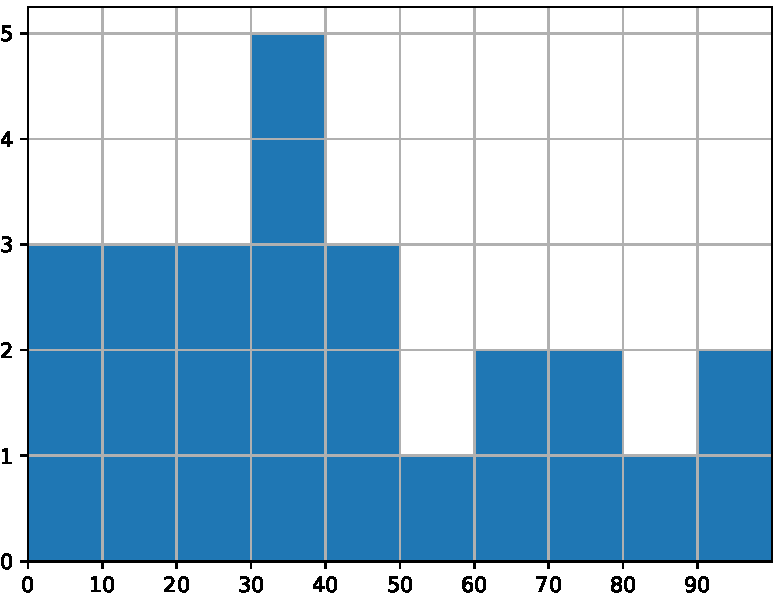
\includegraphics[width=\textwidth]{fig/histogram.pdf}
				\caption{Histogramm}\label{fig:1a}		
			\end{subfigure}
			\quad
			\begin{subfigure}[t]{.45\textwidth}
				\centering
				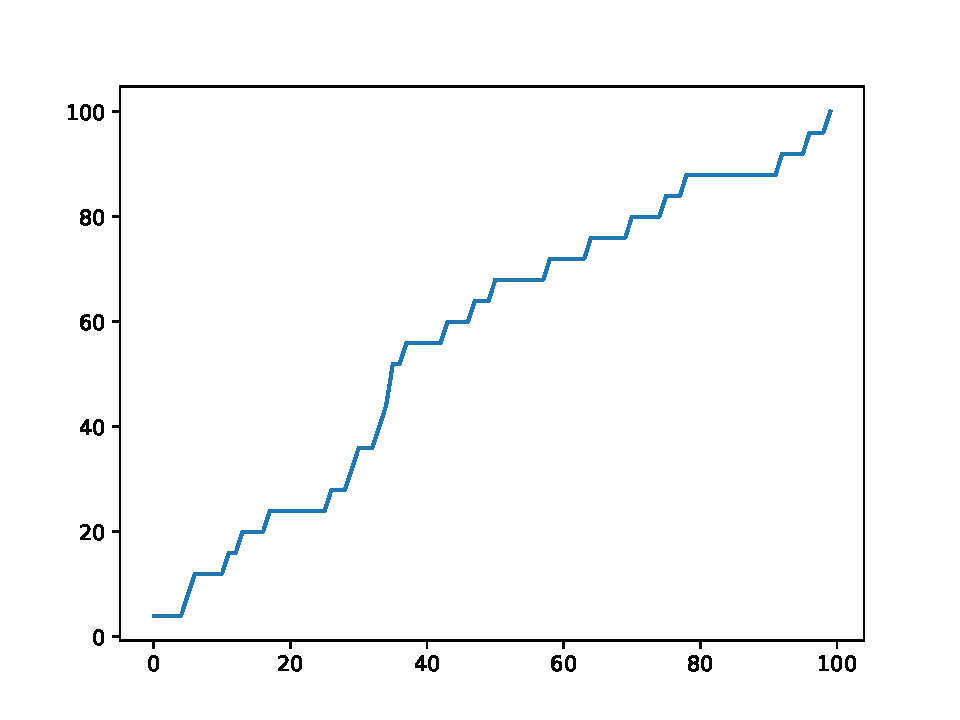
\includegraphics[width=\textwidth]{fig/s-curve.pdf}
				\caption{S-Kurve}\label{fig:1b}
			\end{subfigure}
			\caption{Plots}\label{fig:1}
		\end{figure}
	\end{frame}
\end{document}
